\title{Mastering the game of Connect 4 through self-play}
\author{
        Julian Wandhoven \\
                FGZ\\
}
\date{\today}

\documentclass[12pt]{article}
\usepackage[dvipsnames]{xcolor}
\usepackage{amssymb}
\usepackage{tabularx}
\usepackage{titlesec}
\usepackage{amsmath}
\usepackage{svg}
\usepackage{caption}
\usepackage{hyperref}
\usepackage{lscape}
\usepackage{import}
\usepackage{caption}
\usepackage{subcaption}
\usepackage{float}
\usepackage{listings}
\usepackage{xcolor}
\usepackage{minted}

\usepackage{rotating}
\usepackage{tikz}

\usepackage{graphicx}
\graphicspath{ {./images/} }

\usepackage[most]{tcolorbox}

\newtcolorbox{memoBox}[1][]{%
  sharp corners,
   colback=white,
  attach title to upper,
  #1
}


\setcounter{secnumdepth}{5}
\setcounter{tocdepth}{5}
\lstset { %
    language=C++,
    backgroundcolor=\color{black!5}, % set backgroundcolor
    basicstyle=\footnotesize,% basic font setting
}



\titleformat{\paragraph}
{\normalfont\normalsize\bfseries}{\theparagraph}{1em}{}
\titlespacing*{\paragraph}
{0pt}{3.25ex plus 1ex minus .2ex}{1.5ex plus .2ex}

\titleformat{\subparagraph}
{\normalfont\normalsize\bfseries}{\thesubparagraph}{1em}{}
\titlespacing*{\subparagraph}
{0pt}{3.25ex plus 1ex minus .2ex}{1.5ex plus .2ex}

\newcommand{\imgRef}[1]{(fig \ref{#1} on page \pageref{#1})}
\newcommand{\equationref}[1]{equation \ref{#1} on page \pageref{#1}}
\newcommand{\sectionref}[1]{section \ref{#1} ``\nameref{#1}'' on page \pageref{#1}}
\newcommand{\listingref}[1]{listing \ref{#1} on page \pageref{#1}}
\newcommand{\source}[1]{\caption*{Source: {#1}} }
\newcommand{\quckeq}[1]{(\ref{#1})}
\newcommand{\quickeq}[1]{\quckeq{#1}}
\newcommand{\InBreadcrums}[0]{e \in \mathbb E_{back,l,L}}

\newcommand{\tickTackToe}[9]{
\begin{tabular}{p{7px}|p{7px}|p{7px}}
\multicolumn{3}{c}{}\\
  #1 & #2 & #3 \\      \hline
  #4 & #5 & #6 \\      \hline
   & #7 & #8\\
\multicolumn{3}{c}{#9}
\end{tabular}
}
\newcommand{\ticTacToe}[9]{
\begin{tabular}{p{7px}|p{7px}|p{7px}}
  #1 & #2 & #3 \\      \hline
  #4 & #5 & #6 \\      \hline
  #7 & #8 & #9 \\
\end{tabular}
}
\newcommand{\rewardArrow}[2]{\(\xrightarrow[= #2]{R(\dots)}\) }

\newcommand{\FittedEloRaiting}{408}
\newcommand{\FittedScoringThreshold}{2.8}
\newcommand{\batchSize}{256}

\newcommand{\mathColor}[2]{\color{#1}#2\color{black}}
\newcommand{\gold}{YellowOrange}

\hypersetup{
    colorlinks=true,
    linkcolor=blue,
    filecolor=magenta,      
    urlcolor=blue,
    pdfpagemode=FullScreen,
    }

\urlstyle{same}

\definecolor{mygreen}{rgb}{0,0.6,0}
\definecolor{mygray}{rgb}{0.5,0.5,0.5}
\definecolor{mymauve}{rgb}{0.58,0.29,0}
\definecolor{codeLightGray}{rgb}{0.9,0.9,0.9}

\lstset{ 
  backgroundcolor=\color{codeLightGray},   % choose the background color; you must add \usepackage{color} or \usepackage{xcolor}; should come as last argument
  basicstyle=\footnotesize,        % the size of the fonts that are used for the code
  breakatwhitespace=false,         % sets if automatic breaks should only happen at whitespace
  breaklines=true,                 % sets automatic line breaking
  captionpos=b,                    % sets the caption-position to bottom
  commentstyle=\color{mygreen},    % comment style
  deletekeywords={...},            % if you want to delete keywords from the given language
  escapeinside={\%*}{*)},          % if you want to add LaTeX within your code
  extendedchars=true,              % lets you use non-ASCII characters; for 8-bits encodings only, does not work with UTF-8
  %frame=single,	                   % adds a frame around the code
  keepspaces=true,                 % keeps spaces in text, useful for keeping indentation of code (possibly needs columns=flexible)
  keywordstyle=\color{blue},       % keyword style
  language=C++,                 % the language of the code
  morekeywords={*,...},            % if you want to add more keywords to the set
  numbers=left,                    % where to put the line-numbers; possible values are (none, left, right)
  numbersep=5pt,                   % how far the line-numbers are from the code
  numberstyle=\tiny\color{mygray}, % the style that is used for the line-numbers
  rulecolor=\color{black},         % if not set, the frame-color may be changed on line-breaks within not-black text (e.g. comments (green here))
  showspaces=false,                % show spaces everywhere adding particular underscores; it overrides 'showstringspaces'
  showstringspaces=false,          % underline spaces within strings only
  showtabs=false,                  % show tabs within strings adding particular underscores
  stepnumber=1,                    % the step between two line-numbers. If it's 1, each line will be numbered
  stringstyle=\color{mymauve},     % string literal style
  tabsize=2,	                   % sets default tabsize to 2 spaces
  %title=\lstname                   % show the filename of files included with \lstinputlisting; also try caption instead of title
}
\newcommand{\incFile}[2]{\label{code:#2}\lstinputlisting[language=#1]{code/#2}}
\newcommand{\incDemo}[2]{\label{demo:#2}\lstinputlisting[language=#1]{demos/#2}}

\begin{document}
\maketitle
\begin{abstract}
%\noindent A reimplementation of the Alpha Zero algorithm in C++ using the PyTorch library, based on the 2 papers by Google Deep Mind~\cite{silver2018general}\cite{silver2017mastering}.
\noindent Alpha Zero is an AI algorithm that is capable of learning to play zero sum stated multiplayer games. These types of games include Go, Chess and so forth. This is done by training a neural network from data generated by a Monte Carlo Tree Search. In this project, I modified and implemented the algorithm from scratch and applied it to Connect4. This document also explains the basic mathematics behind neural networks and Monte Carlo Tree Searches. (see articles \cite{silver2018general}\cite{silver2017mastering})
\end{abstract}
\newpage
\tableofcontents
\newpage

Alpha Zero is an algorithm published in 2018 by Google Deepmind as the generalization of AlphaGo Zero, an algorithm that learned to play the game of Go using only the rules of the game. In the generalized version, the same principles were applied to Chess and Shogi. Unlike previous algorithms such as StockFish or Elmo that use hand-crafted evaluation functions along with alpha-beta searches over a large search space, Alpha Zero uses no human knowledge. Rather, it generates all information through self-play. It has been shown to achieve superhuman performance in Chess, Shogi and Go. In this project, an AI will be built and taught to play connect4. The entire algorithm is implemented in C++. Starting from a random computer player (agent), the algorithm is able to improve that agent, and in so doing create a better one. This can be repeated to produce a series of agents, that become progessively better at playing the game. These agents will then be evaluated against each other using the Elo evaluation system \cite{elo1978rating} (see \sectionref{sec:evaluation}). Additionally, I have added a short introduction on the mathematics behind neural networks in \sectionref{NN}. 

\section{Methods}
\label{Methods}
The Alpha Zero algorithm is a reinforcement learning algorithm using two major parts: a) a {\it Monte Carlo tree search} (MCTS) that is guided by b) the {\it neural network} to improve performance.
The agent runs a certain amount of simulation games using its MCTS and neural network. At each step, the MCTS evaluates the most promising next states as given by the neural network's estimation. The MCTS, by simulating games starting from the current state, will improve the neural network's prediction for that state. At the end of each game, the winner is determined and used to update the neural network's estimation of who would win a game starting from a certain state. Training an AI by teaching it to prefer advantagious actions is called reinforcement learning.
\subsection{Reinforcement Learning}
When training neural networks, there are three major possible situations: Supervised learning, unsupervised learning, and reinforcement learning. The first uses predetermined data with known in- and outputs the network is trained to predict. An example of supervised learning is the recognition of handwriting as the data is defined by humans. This method consists of creating a large database of examples, and the neural network is then trained to predict a given output for all examples. 

Unsupervised learning or self-organization is used when there is no previously available data and the neural network has to create those classifications itself. An example of unsupervised learning is Vector quantization. The algorithm sorts points in n-dimensional space into a predetermined amount of groups. Each group is defined by its centroid point and contains all points closer to that centroid point than any other centroid point. Training happens by selecting a random sample point from the input data, and moving the closest centroid point towards this sample point by a fraction of the distance between them.\cite{wiki:Vector_quantization} This is repeated untill an equilibrium is reached. An example of both supervised and unsupervised learning can be seen in the demo\footnote{demo is at \url{https://github.com/JulianWww/Matura-AlphaZero-demos}}.

These two methods represent the extreme ends of the spectrum. Reinforcement learning can be thought of as an intermediate form. It uses a predetermined environment which gives positive, neutral and negative feedback. The neural network is then discouraged from taking actions leading to negative feedback and encouraged to take actions leading to positive feedback. The feedback is determined by the environment the agent learns to interact with. In this case, losing a game would be bad and result in negative feedback whereas winning a game leads to positive feedback. Ties lead to neutral feedback. The agents learning is set up in such a way, that it is encouraged to take actions leading to positive feedback and discouraged from taking actions that lead to negative feedback. However, actions can lead to feedback that only occurs many game steps ahead in the future. A common approach to solve this problem is to have the feedback propagate backwards to previous actions. In Alpha Zero, this is handled by the memory (see \sectionref{sec:memory}). When the game reaches an end state and a winner is determined, the feedback is propagated backwards up through all states used to get to that end state. If the player won, the feedback is positive. If he lost, it is negative. More specifically, if a player takes an action \(a_s\) at a state \(s\), that leads to a win for that player, the reward for that state is defined as \(R(s,a_s) = 1\). On the other hand, if the action leads to a loss, the reward will be \(R(s, a_s) = -1\). If the game ends in a tie, the reward is \(R(s,a_s) = 0\). Every agent \(p\) will try to maximize \(\sum_{s\in g\cap p} R(s, a_s)\). \(g\cap p\) is the set of all states in which the player \(p\) takes an action during the game \(g\). Let's look at a tic tac toe example of the following game:
\begin{center}
\tickTackToe{}{}{}{}{}{}{}{}{player X} \to \tickTackToe{X}{}{}{}{}{}{}{}{player O} \to \tickTackToe{X}{O}{}{}{}{}{}{}{player X} \to \tickTackToe{X}{O}{}{}{X}{}{}{}{player O} \to \tickTackToe{X}{O}{}{O}{X}{}{}{}{player X} \to \tickTackToe{X}{O}{}{O}{X}{}{}{X}{}
\end{center}
Since player \(X\) won the game, the reward for every state \(s\in g\cap X\) is \(R(s, a_s) = 1\) and the reward for every state \(s\in g\cap O\) is \(R(s, a_s) = -1\). The reward for the entire game is:
\begin{center}
\tickTackToe{}{}{}{}{}{}{}{}{} \rewardArrow{X}{1} \tickTackToe{X}{}{}{}{}{}{}{}{} \rewardArrow{O}{-1} \tickTackToe{X}{O}{}{}{}{}{}{}{} \rewardArrow{X}{1} \tickTackToe{X}{O}{}{}{X}{}{}{}{} \rewardArrow{O}{-1} \tickTackToe{X}{O}{}{O}{X}{}{}{}{} \rewardArrow{X}{1} \tickTackToe{X}{O}{}{O}{X}{}{}{X}{}
\end{center}
\begin{memoBox}
The important thing to keep in mind is that reinforcement learning algorithms encourage actions that lead to a positive feedback and discourage actions that lead to a negative feedback.
\end{memoBox}
\subsection{Game}
In order to train a reinforcement learning AI, it must interact with an environment. In Alpha Zero the game is the environment. The game consists of a series of constant unchanging game states. Every game state consists of a game board and a player. An end game state is a state at which the game is over. Every game ends in an end game state. At an end game state, one player won or the game ended in a tie. Together, the successive states form a directed graph. Any possible path through this graph starting from a root state (the inital state of the board) and ending in any end game state, is a possible game. From an end game state, there is nowhere left to go.
For connect4 an end game state has either four stones in a line or a full game board.
Let \(\mathbb{G}\) be the set of all legal game states.
Let \(\mathbb{G}_{done} \subset \mathbb G\) be the set of all game states for which the game is over. At every game state one player is at turn. This means that that player will take an action next. Let \(\phi(s)~:~\mathbb{G}\to\{1,-1\}\) be the function mapping states to players. In the tick-tack-toe example from earlier we could say that:
\begin{align}
\phi(s) = \left\{\begin{matrix}
1 & s \in g\cap X\\
-1 & s \in g\cap O
\end{matrix}\right.
\end{align}
More generally, \(\phi(s) = 1\) if the first player (the player that starts the game) is at turn and \(\phi(s) = -1\) if the other player is a turn.

\subsubsection{Game Board}
Board games consist of placing stones of different types on a board with a certain amount of fields. Many games, like Go, Chess and Connect4, arrange their fields in a rectangular pattern. These games have two distinct stones. We can represent these game boards as a stack of binary layers. Every layer is associated with one kind of stone. Each layer contains a one, where the board has a stone of the appropriate type and zeros everywhere else. For instance, the following tic tac toe game board can be represented by the following binary layers stack.\[
\ticTacToe{}{X}{O}{O}{X}{}{O}{}{X}\to
\left[ 
\begin{bmatrix}
0 & 1 & 0 \\
0 & 1 & 0 \\
0 & 0 & 1 \\
\end{bmatrix}
\begin{bmatrix}
0 & 0 & 1 \\
1 & 0 & 0 \\
1 & 0 & 0 \\
\end{bmatrix}
\right]
\] 
Internally, the game board is represented by a flat vector. The conversion from a game state \(s  \in \mathbb G\) to a vector is defined as \(vec(T_s(s))\). Where \(T_s(s):\mathbb G \to \mathbb R^{\cdots}\) is the board's 3-dimensional board tensor. The \(vec\) function is defined in \sectionref{sec:ref:vectorization:tensor}.
\begin{equation}
vec
\left(\left[ 
\begin{bmatrix}
a_{111} & \cdots & a_{11o} \\
\vdots & \ddots & \vdots \\
a_{1n1} & \cdots & a_{1no} \\
\end{bmatrix}
\cdots
\begin{bmatrix}
a_{m11} & \cdots &  a_{m1o} \\
\vdots   & \ddots & \vdots   \\
a_{mn1} & \cdots & a_{mno}  \\
\end{bmatrix}
\right]\right) = \left(\begin{matrix}
a_{111}      \\
\vdots        \\
a_{11o}      \\
\vdots        \\
a_{1n1}      \\
\vdots        \\
a_{1no}      \\
\vdots        \\
a_{m11}     \\
\vdots        \\
a_{m1o}     \\
\vdots        \\
 a_{mn1}    \\
\vdots        \\
 a_{mno}    \\
\end{matrix}\right)
\end{equation}
This operation for the tic tac toe board from above would look like this:
\begin{equation}
vec\left(T_s\left(\ticTacToe{}{X}{O}{O}{X}{}{O}{}{X}\right)\right) = 
[0\,1\,0\,0\,1\,0\,0\,0\,1\,0 \,0 \,1\,1\,0\,0\,1\,0\,0]^T
\end{equation}
\subsubsection{Actions}
Actions are numbers used to identify changes to the game. Every game has a set of all possible actions represented by numbers \(\mathbb{A}_{possible} \subset \mathbb{N}_0\). In connect4, the set of all possible actions for the current player is \(\mathbb{A}_{possible} = [0, 41]\cap\mathbb N\). There is no need to have actions for the player, that is not at turn as these will never be taken. Every number is associated with a position on the game board. The mapping of actions to game fields is as follows for connect4:
\begin{center}
\begin{tabular}{| c | c | c | c | c | c | c |}
 \hline
0 & 1 & 2 & 3 & 4 & 5 & 6  \\\hline
7 & 8 & 9 & 10 & 11 & 12 & 13\\\hline
14 & 15 & 16 & 17 & 18 & 19 & 20 \\\hline
21 & 22 & 23& 24 & 25 & 26 & 27 \\\hline
28 & 29 & 30 & 31 & 32 & 33 & 34 \\\hline
35 & 36 & 37 & 38 & 39 & 40 & 41 \\\hline
\end{tabular}
\end{center}
Let \(\mathbb{A}(s)\) be the set of all legal actions for a given state  \(s \in \mathbb{G}\). For all states \(s_{done} \in \mathbb{G}_{done}\) the set of all legal actions \(\mathbb{A}(s_{done})\) is the empty set. The function \(\mathcal{A}~:~\mathbb{G}\times\mathbb{A}\to\mathbb{G}\) is used to get from one game state to another by taking an action. Where \(\mathbb A\) is the set of all legal actions for the chosen game state. If we were to map actions to positions for tic tac toe as follows and the current game state were
\begin{center}\begin{tabular} { c c }
\begin{tabular}{| c | c | c |}
 \hline
 0 & 1 & 2 \\\hline
 3 & 4 & 5 \\\hline
 6 & 7 & 8 \\\hline
\end{tabular} & \tickTackToe{X}{O}{}{}{}{}{}{}{State \(s\)}
\end{tabular}\end{center}
then player \(X\) is allowed to place a stone in any empy field \(\implies\mathbb A(s) = \left\{ 2, 3, 4, 5, 6, 7, 8 \right\}\). Therefore, \(\mathcal A(s, a)\) is valid if \(a \in \mathbb A(s)\) and otherwise invalid.

\subsection{MCTS \cite{chaslot2008parallel}\cite{silver2018general}}
A Monte Carlo tree search (MCTS) is a tree search algorithm that can be used to find sequences of actions leading to a desirable outcome. This is done by procedurally generating a directed graph of possible successor states to the current state or root state. In Alpha Zero it is used to improve the neural network's prediction.
Because an MCTS changes during simulation, indices are used to specify which simulation step the tree is in. An MCTS simulation consists of three phases: \nameref{sec:Methods:MCTS:Leaf_selection}, \nameref{sec:Methods:MCTS:Node Evaluation and Expansion} as well as \nameref{sec:Methods:MCTS:Backfill}.

A MCTS graph consists of nodes and edges. Nodes represent game states and edges represent actions. As in the game, edges connect nodes to each other.
The amount of nodes and structure of the MCTS is changed by the algorithm itself during simulation. During the first simulation, the tree contains only the root node \(n_0\). The root node is the starting point of the simulation. Let \(l \in \mathbb L\) be the index of the current simulation step. Let \(\mathbb L = \mathbb [0, S]\cap\mathbb N\) be the set of all \(l\), where \(S\) is a constant defined in the algorithm's configuration file. Let \(\mathbb{M}_l \subseteq \mathbb{G}\) be the set of all nodes in the tree at step \(l\in\mathbb L\). That implies \(\mathbb M_0 = \left\{n_0\right\}\).

 Every node \(n_l \in \mathbb{M}_l\) has a set of edges \(\mathbb{E}_l(n_l)\) at step \(l\) that point from it to another node. Let \(\mathbb{E}_l\) be the set of all edges in the current graph. The function \(\mathcal{N}_{to_l}~:~\mathbb{E}_{l}\to\mathbb{M}_l\) maps an edge to the node it is pointing to while \(\mathcal{N}_{from_l}~:~\mathbb{E}_{l}\to\mathbb{M}_l\) is used to find the node an edge is pointing from.
Furthermore, it is useful to distinguish expanded nodes from leaf nodes. Leaf nodes are nodes that don't have edges leading out of them. Let \(\mathbb{M}_{leaf_l} \subseteq \mathbb{M}_l\) be the set of leafnodes. For every node \(n_l\in \mathbb{M}_{leaf_l}\), the following is true by definition \(\mathbb{E}_l(n_l) = \emptyset\). Expanded nodes have edges leading out of them.

\begin{figure}[H]
  \centering
  \includesvg[height=.25\textheight]{images/mctsExample}
  \captionsetup{width=.9\linewidth}
  \caption{This is a possible MCTS graph. In this exampel the set of all nodes is \(\mathbb M = \{n_1, n_2,\hdots,n_8\}\), the set of all leaf nodes is \(\mathbb M_{leaf} =  \{n_3, n_5, n_6, n_7, n_8\}\). The set  \(\mathbb E(n)\) of a node \(n\), beeing the set of edges pointing away from that node, for node \(n_1\) is \(\mathbb E(n_1) = \{e_1, e_2,e_3\}\). The same for all other nodes. \(\mathcal N_{to}(e)\) is the node an edge \(e\) points to. This means that \(\mathcal N_{to}(e_1) = n_3\), \(\mathcal N_{to}(e_2) = n_2\), etc. In contrast \(\mathcal N_{from}(e)\) is the node an edge \(e\) points from. Therefore, \(\mathcal N_{from}(e_1) = n_1, \mathcal N_{from}(e_2) = n_1\), etc.}
	\label{fig:mcts:example}
\end{figure}

\subsubsection{Evaluation Basis}
The MCTS's goal is to find a good estimation of the reward for a certain action at a certain state. This reward estimation is \(Q_l~:~\mathbb{E}_{l}\to \mathbb{R}\). To define \(Q_l\), the functions \(W_l~:~\mathbb{E}_{l}\to\mathbb{R}\) and \(N_l~:~\mathbb{E}_{l}\to\mathbb{N}_0\) are required. \(N_l(e_l)\) is the amount of times an edge \(e_l\in\mathbb{E}_{l}\) has been traversed during simulation. \(W_l(e_l)\) is the sum of the reward computations from all \(N_l(e_l)\) times the edge has been evaluated. With these two functions \(Q_l\) is defined as:
\begin{equation}\label{eq:Ql}
Q_l(e_l) = 
\begin{cases}
0 & N_l(e_l) = 0\\
\frac{W_l(e_l)}{N_l(e_l)} &
\end{cases}
\end{equation}
In a classic MCTS this is all that would be required. However, Alpha Zero uses an improved MCTS that increases computational efficency by exploring more promissing paths more early on. In order to accomplish this, the neural network gives an estimation of the advantagiousness of a certain action at a certain state. This estimation is the edges policy \(P_l~:~\mathbb E_l \to \mathbb R\). The policy approximates
\begin{equation}
\frac{N_{mean}(e_l)}{\sum_{e\in\mathbb E_l(\mathcal N_{from}(e_l))} N_{mean}(e)}
\end{equation}
where \(N_{mean}\) is the average \(N_S\) over all previous simulations.

\subsubsection{Leaf Selection} \label{sec:Methods:MCTS:Leaf_selection}
MCTS's evaluation starts by simulating future moves within the tree. This is done by selecting an edge and then following that edge to a new node. From there, the next edge and node are selected. This is repeated until a leaf node is reached. To select an edge and thus a node from the current node \(n_l\in \mathbb{M}_l\) the selection function \(\sigma_l~:~\mathbb M_l \to\mathbb E_l\) is used. To define \(\sigma_l\) we must first define the edge evaluation function \(u_l~:~\mathbb{E}_{l}\to\mathbb{R}\). \(u_l\) is defined as:
\begin{equation}
u_l(e) = Q_l(e) + c \cdot P_l(e)\cdot\frac{\sqrt{\Sigma_{b\in\mathbb{E}(\mathcal{N}_{from_l}(e))}N_l(b)}}{1+N_l(e)}
\end{equation}
where \(c\in \mathbb{R}^+\) is the exploration constant used to define how important exploration is. The smaller \(c\) is, the more important is \(Q\) and the less important are exploration and \(P\). For my configuration \(c = 2\) turned out to work fine. \(\sigma_l\), for a given node \(n_l\in\mathbb{M}_l\), is then defined as:
\begin{equation}\label{eq:sigma}
\sigma_l(n_l) = \text{argmax}_l(\mathbb{E}_l(n_l))
\end{equation}
\(\text{argmax}_l\) returns the edge \(e \in\mathbb E_l\) with the largest \(u_l(e)\).\\
In order to find a leaf node \(n_{L_l}\) starting from the root node \(n_{0_l}\) and to be able to update the tree later on, the following algorithm is run until a leaf node is found. First, let \(i \in\mathbb N_0\) be the index of the iteration of this algorithm. Let \(\mathbb E_{back,l,i} \subseteq \mathbb E_l\) be the set of edges traversed by the algorithm at step \(i\) during simulation \(l\). By definition \(\mathbb E_{back,l,0} := \emptyset\). Then:
\begin{align}
n_{(i+1)_l} &= \mathcal N_{to}(\sigma_l (n_{i_l}))\\
\mathbb E_{back,l,i+1} &= \mathbb E_{back,l,i} \cup \{\sigma_l (n_{i_l})\}
\end{align}
Once a leaf-node \(n_{L_l}\in\mathbb{M}_{leaf_l}\) is reached at step \(i = L\) that node is evaluated. \(\mathbb E_{back,l,L}\) will be important in \sectionref{sec:Methods:MCTS:Backfill}. 


\subsubsection{Node Evaluation and Expansion}
\label{sec:Methods:MCTS:Node Evaluation and Expansion}
When a leaf node \(n_{L_l}\) is reached, there are two possible cases. Either \(n_{L_l}\) is an end game state or not.
\paragraph*{case: end game state \(n_{L_l} \in \mathbb G_{done}\)}
In this case, the tree is not changed but backfill is performed with the reward value \(v_l \in \{0, \pm 1\}\):
\begin{equation}
v_l = -R(n_{(L-1)_l}, e)
\end{equation}
where \(e\) is the edge taken at node \(n_{(L-1)_l}\) to reach \(n_{L_l}\). \\
(The value of \(v_l\) is ``negative'' because it is player B's turn after player A won.)

\paragraph*{case: not end game state \(n_{L_l} \not\in \mathbb G_{done}\)}
In this case, the node is passed to the neural network (\sectionref{NN}). The neural network evaluates the node and outputs a policy vector \(\pi_l \in [0,1]^{|\mathbb A|}\) and an estimated reward scalar \(v_l \in \mathbb [-1,1]\). \(\pi_l\) is the estimation of the advantageousness of every action in \(\mathbb A\). After evaluation, the leaf node is expanded.
Let \(\mathbb E_{new}\) be the next set of all edges pointing away from \(n_{L_l}\). This set contains one edge for every action in \(\mathbb A(n_{L_l})\).
Let \(\mathbb M_{new}\) be the set of nodes, that the edges in \(\mathbb E_{new}\) are pointing to.
The various tree sets and functions are then updated as follows for step \(l+1\).
\begin{align}
\mathbb M_{l+1}   =& \mathbb M_l \cup \mathbb M_{new} \\
\mathbb E_{l_+1}  =& \mathbb E_l  \cup \mathbb E_{new} \\
%
\mathbb E_{l+1}(n) &= 
\left\{
\begin{matrix}
\mathbb E_{new} & n = n_{L_l}\\
\emptyset & n \not\in\mathbb M_l\\
\mathbb E_l(n)
\end{matrix}
\right.\\
%
\mathbb M_{leaf_{l+1}} &= \left\{n\in\mathbb M_{l+1}~:~\mathbb E_{l+1}(n) = \emptyset\right\}\\
%
P_{l+1}(e) &= 
\left\{
\begin{matrix}
P_l (e) & e \in\mathbb E_l\\
\pi_{l_e}&
\end{matrix}
\right.
\end{align}



\subsubsection{Backfill}
\label{sec:Methods:MCTS:Backfill}
%Let \(\mathbb E_{traversed}_l\) be the set of all edges traversed during leaf selection.
The reward value \(v_l\) is used to update the \(P\), \(W\) and \(Q\) function as follows for every edge \(e\in\mathbb E_{l+1}\):
\begin{align}
N_{l+1}(e) &= \left\{\begin{matrix}
0 & e \in\mathbb E_{new}\\
N_l(e)+1 & \InBreadcrums\\
N_l(e)
\end{matrix}\right.\\
%
W_{l+1}(e) &= \left\{\begin{matrix}
0 & e \not\in\mathbb E_l\\
W_l(e)+v_l\cdot\phi(n_{L_l})\phi(\mathcal N_{from}(e)) & \InBreadcrums\\
W_l(e)
\end{matrix}\right.
\end{align}
The ``\(\phi\) multiplication'' \(\phi(n_{L_l})\phi(\mathcal N_{from}(e)) = \pm 1\) is needed to reward the moves of the winning player and  to punish the moves of the other player.


\noindent\(Q_{l+1}\) is already defined according to \quckeq{eq:Ql}. In contrast to \cite{silver2018general}, this implementation stores the MCTS simulation values in the edges to allow for the fact that actions from two different nodes leading to the same node are not identical and therefore should not be treated as such. But nodes of the same game state are identical and should be treated as such.\\\\
%-------------------------------------------------------------------------
\subsection{Neural Network}
Search algorithms like MCTS are able to find advantageous action sequences. Traditionally, like in ``stockfish 8'' for example, the search algorithm is improved by using evaluation functions. These functions are generally created using human master knowledge. In the Alpha Zero algorithm, this evaluation function is instead a biheaded deep convolutional neural network trained by information gathered from MCTS simulations. In order to understand the training process, one must first understand how the neural network functions.
\label{NN}
\subsubsection{Introduction to Neural Networks}
An artificial neural network or just neural network is a mathematical function inspired by biological brains. Although there are many types of neural networks, the only relevant one to this work is the feed forward network. These models consist of multiple linear computational layers separated by non-linear activation functions. Every layer takes the outputs of the previous layer, and applies a linear transformation to it~\cite{zhang2018artificial}. There are many different feed-forward neural network layers and activation functions to chose from when designing a neural network. To focus this explanation, only the relevant ones will be discussed along with the back-propagation algorithm.
\paragraph{Fully Connected Layer}
A fully connected layer is the most basic layer. It applies a simple matrix multiplication. The layer takes a \(1 \times n\) dimentional matrix \(x \in \mathbb{R}^{1\times n}\) as an input and multiplies it by a weight matrix \(w \in\mathbb{R}^{n\times m}\). This operation outputs a \(1\times m\) dimensional matrix to which a bias \(b \in \mathbb{R}^{1 \times m}\) is added to form the output matrix \(v \in \mathbb{R}^{1 \times m}\) containing the output values of the layer. \(v\) is then fed to the next layer. The addition of the bias vector \(b\) is optional. In some situations it is worth dropping the bias in favour of computational speed. The fully connected layer forward propagation function shall be defined as \(\delta_{wb}~:~\mathbb{R}^n\to\mathbb{R}^m\)
\begin{equation} \label{eq:NN:fully_connected_layer_forward}
\delta_{wb}(x) = w \cdot x + b
\end{equation}

\paragraph{Convolutional Layer}
Convolutional layers are commonly used for image processing. They are used here to perform image processing of the ``image'' of the game board. Their input is a 3d-tensor \(I \in \mathbb R^{i\times j\times l}\). They perform the same operations over the entire image searching for certain patterns. In order to achieve this, a set of kernels \(\mathbb{K}\) of size \(m\times n\) is defined for the layer. Every kernel \(k\in\mathbb K\) consists of a weight tensor \(w_k \in \mathbb R^{m\times n\times l}\) and an optional bias scalar \(b_k \in\mathbb R\).
These kernels are then placed over every possible location of the input tensor \(I\), and an output is computed for that position and kernel. This is useful to recognize patterns, that are independant of location. For every kernel \(k\in \mathbb{K}\), the kernel's forward operation \(\xi_k~:~\mathbb{R}^{m \times n \times l}\to\mathbb{R}\) is defined as:
\begin{equation}\label{eq:NN:kernelOpperation}
\xi_k(I_{sub}) = w_k \diamond I_{sub} + b_k
\end{equation}
where \(\diamond\) is the Tensor inner product defined in \equationref{eq:defs:Inner_product_3d} and \(I_{sub}\) is a subtensor of \(I\).
The convolutional operation \(\Lambda~:~\mathbb{R}^{i\times j \times l}\to\mathbb{R}^{i-m+1 \times j-n+1 \times |\mathbb{K}|}\) is an element wise opperation. Given that  \(I \in \mathbb{R}^{i\times j\times l}\) is the layer input, every element of \(\Lambda(I)_{abc}\) with \(a \in [1, i-m+1]\cap\mathbb N\), \(b \in [1, j-n+1]\cap\mathbb N\) and \(c \in [1, |\mathbb{K}|]\cap\mathbb N\) is defined as:
\begin{equation}\label{eq:NN:convolutional_opperation}
\Lambda(I)_{abc} = \xi_{k_c}(\left<I\right>_{m\times n,\,ab})
\end{equation}
where \(k_c\) is the c\textsuperscript{th} kernel and \(\left<\right>\) is the submatrix operation as defined in \sectionref{sec:Ref:submatrix}.
\\\\\noindent
For example, given the following input tensor \(I \in\mathbb{R}^{4\times4\times1}\): % matrix slice
\[
I = \left[
\begin{matrix}
[3] & [0] & [1] & [5] \\
[2] & [6] & [2] & [4] \\
[2] & [4] & [1] & [0] \\
[3] & [0] & [1] & [5] \\
\end{matrix}
\right]
\]
and the following kernel weight matrix \(w_k \in \mathbb{R}^{3 \times 3 \times 1}\) along with the scalar \(b\in \mathbb{R}\),
\begin{align*}
w_k &= \left[
\begin{matrix}
[-1] & [0] & [1] \\ 
[-2] & [0] & [2] \\
[-1] & [0] & [1]
\end{matrix}
\right]\\
b &=7\\
\end{align*}
there are four possible locations in which \(w_k\) can be placed within \(I\). As there is only one kernel, the length of the set of all kernels \(|\mathbb{K}| = 1\). This also means that \(\Lambda(I) \in R^{2 \times 2 \times 1}\). To calculate \(\Lambda(I)_{111}\), we compute the kernel operation \(\xi_{k_1}(\left<I\right>_{S_{3\times 3,\,11}})\)
\begin{equation}
\label{eq:conv:eg}
\Lambda
\left(\begin{bmatrix}
[3] & [0] & [1] & [5] \\
[2] & [6] & [2] & [4] \\
[2] & [4] & [1] & [0] \\
[3] & [0] & [1] & [5] \\
\end{bmatrix}\right)_{111}\\
 = \begin{bmatrix}
[3] & [0] & [1] \\
[2] & [6] & [2] \\
[2] & [4] & [1] \\
\end{bmatrix}\diamond
\begin{bmatrix}
[-1] & [0] & [1] \\
[-2] & [0] & [2] \\
[-1] & [0] & [1]
\end{bmatrix} + 7
\end{equation}
\begin{align*}
&= -1 \cdot 3 + 0 \cdot 0 + 1 \cdot 1 - 2 \cdot 2 + 0 \cdot 6 + 2 \cdot 2 -1 \cdot 2 + 0 \cdot 4 + 1 \cdot 1 + 7\\
&= 4\\
\end{align*}
The same is done for \(\Lambda(I)_{121}\), \(\Lambda(I)_{211}\) and \(\Lambda(I)_{221}\). This leads to a \(\Lambda(I)\) of:
\[
\Lambda(I) = \begin{bmatrix}
[4] & [3] \\
[4] & [2] \\
\end{bmatrix}
\]
\paragraph{Activation Function}
All neural network layers are linear functions. Thus, given two layer evaluation functions \(f_1(x) = ax + b\) and \(f_2(x) = cx + d\), the chained function \(f(x) = f_1(f_2(x))\) is also linear.
In order to represent non linear functions, a non linear activation function \(f_a\) is added between two neural network layers. Thus, the chained function becomes \(c(x) = f_1(f_a(f_2(x)))\). In this neural network, three different activation functions are used: \(tanh\), \(softmax\), and \(LeakyReLU\). These functions are defined as follows:
\subparagraph*{tanh:}\(\mathbb{R}\to \mathbb{R}\)

\begin{center}
\includesvg[width=0.9\columnwidth]{images/tanh}
\captionof{figure}{tanh function in blue and the tanh's derivative is in orange}
\end{center}

\begin{align} \label{eq:NN:tanh}
tanh(x) &= \frac{e^x-e^{-x}}{e^x+e^{-x}}\\
\label{eq:NN:tanh_derivative}
\frac{d}{dx}tanh(x) &= sech(x)^2
\end{align}\\
Therefore, for a given vector \(v \in \mathbb R^n\), \(tanh(v)\) shall be defined as:
\begin{equation}\label{eq:vecTanh}
tanh(v) = \left(
\begin{matrix}
tanh(v_1)\\
tanh(v_2)\\
\vdots\\
tanh(v_n)
\end{matrix}
\right)
\end{equation}
For simple use later on, the derivative of \(tanh(v)\), \(tanh'(v) \in \mathbb R^{n \times n}\) shall be a \(n \times n\) dimensional matrix, defined as
\begin{equation}
tanh'(v)_{ij} = \left\{\begin{matrix}
tanh'(v_{ij}) & i = j \\
0
\end{matrix}\right.
\end{equation}
for every element \(i,j\) in the derivative matrix.

\subparagraph*{softmax:} \(\mathbb{R}^n\to \mathbb{R}^n\)\\
\indent For a given input vector \(v \in \mathbb{R}^n\), the output vector \(o \in \mathbb{R}^n\) at every position \(i \in [1, n]\cap\mathbb N\) is:
\begin{equation} \label{eq:NN:softmax}
o_i = softmax(v)_i = \frac{e^{v_i}}{\sum_{j \in v} e^j}
\end{equation}
\begin{figure}[H]
\centering
\begin{subfigure}{.4\textwidth}
  \centering
  \includesvg[height=.25\textheight]{images/softmaxx}
  \caption{\(o_1\)}
  \label{fig:sub1}
\end{subfigure}%
\begin{subfigure}{.4\textwidth}
  \centering
  \includesvg[height=.25\textheight]{images/softmaxy}
  \caption{\(o_2\)}
  \label{fig:sub2}
\end{subfigure}
\begin{subfigure}{.1\textwidth}
  \centering
  \includesvg[height=.25\textheight]{images/softmaxscale}
  \caption*{scale}
\end{subfigure}
\caption{Graph of the softmax function from \(\mathbb R^2 \to \mathbb R^2\).}
\label{fig:test}
\end{figure}

Because the function's in- and outputs are n dimensional vectors, the derivative is an \(n\times n\) dimensional matrix. When taking its derivative, \(\frac{d}{dv_j}softmax(v)_i\), there are two possible cases. 
\\\indent case \(j = i\):
\begin{equation}
\frac{d}{dv_j}\left[\frac{e^{v_i}}{\sum_{b\in v} e^{b}}\right] = softmax(v)_i\cdot (1 - softmax(v)_j)\\
\end{equation}
\\\indent case \(j \neq i\):
\begin{equation}
\frac{d}{dv_j}\left[\frac{e^{v_i}}{\sum_{b\in v} e^{b}}\right] = -softmax(v)_i\cdot softmax(v)_j \\
\end{equation}
Therefore, the derivative of the softmax function is:
\begin{equation}\label{eq:NN:softmax_derivative}
softmax'(v)_{ij} = \left\{
\begin{array}{ll}
 softmax(v)_i\cdot (1-softmax(v)_j) & i = j\\
 - softmax(v)_i \cdot softmax(v)_j     & i \neq j
\end{array}
\right.
\end{equation}
\subparagraph*{LeakyReLU:}\(\mathbb{R} \to \mathbb{R}\)
\begin{center}
\includesvg[width=0.9\columnwidth]{images/LeakyReLU}
\captionof{figure}{LeakyReLU with \(c = 0.3\)}
\end{center}

\begin{align} \label{eq:NN:ReLU}
\text{LeakyReLU}(x)& = \left\{
\begin{array}{ll}
x & x \ge 0 \\
x \cdot c & x < 0 \\
\end{array}
\right.\\\label{eq:NN:Relu_derivative}
\text{LeakyReLU}'(x) &= \left\{
\begin{array}{ll}
1 & x > 0 \\
c & x < 0 \\
\end{array}
\right.
\end{align}
\(c\) is a constant describing the slope of the function for negative input values. The derivative of the LeakyReLU function is undefined for \(x=0\). However, as we will be performing gradient descent on these functions the derivative must befined for all \(x \in \mathbb R\). A possible definition that accomplishes the objective is:
\begin{equation}
g(x) = 
\begin{cases}
1 & x \ge 0\\
c & x < 0\\
\end{cases}
\end{equation}
Therefore, for a given vector \(v \in \mathbb R^n\), \(\text{LeakyReLU}(v)\) shall be defined as:
\begin{equation}\label{eq:vecTanh}
\text{LeakyReLU}(v) = \left(
\begin{matrix}
\text{LeakyReLU}(v_1)\\
\text{LeakyReLU}(v_2)\\
\vdots\\
\text{LeakyReLU}(v_n)
\end{matrix}
\right)
\end{equation}
For simple use later on, the derivative shall be a \(n \times n\) dimensional matrix, defined as
\begin{equation}
\text{LeakyReLU}'(v)_{ij} = \left\{\begin{matrix}
g(v_{ij}) & i = j \\
0
\end{matrix}\right.
\end{equation}
for every element \(i,j\) in the derivative matrix.


\paragraph{Training introduction} 
To make this explanation easier, I will use a fully connected neural network and assume we are using supervised learning.
Neural network training or backpropagation can be mathematically expressed as minimizing a loss function  \(\ell(Y_{pred}, Y_{true})\) describing how inaccurate the network is. In our case, \(\ell\) takes the neural network's predicted value vector \(Y_{pred}\) and the correct value vector \(Y_{true}\). \(Y_{true}\) must be known before the computation begins. In AlphaZero, \(Y_{true}\) is generated by the MCTS. As with the activation function, there are many different possible loss functions. In this implementation, the mean-square-error (\(mse =\ell\)) loss function is used. \(\ell:~\mathbb R^\mu\times\mathbb R^\mu \to \mathbb R\) is defined as:
\begin{equation} \label{eq:NN:loss_mse}
\ell(Y_{pred}, Y_{true}) = \frac{|Y_{pred} - Y_{true}|^2}{\mu}
\end{equation}
The network then performs gradient descent to find parameters that minimize \(\ell\).  Let \(\ell'~:~\mathbb R^\mu \times \mathbb R^\mu \to \mathbb R^\mu\) be the derivative of \(\ell\).
\begin{equation}\label{eq:lossDerivative}
\ell'(Y_{pred}, Y_{true}) = \frac{2}{\mu} \left(Y_{pred} - Y_{true}\right)
\end{equation}
Given a neural network consisting of \(n\) layers, training will start at the last layer and propagate throught the network from back to front. Hence the name backpropagation. To improve the parameters \(w, b\) (weight and bias) of every layer in the network, the algorithm must determine in which direction and by how much the variables should be moved. Let \(j \in \mathbb N_0\cap [0,n[\) be the index of the layer. The indices start at the first layer (\(j=0\)) and count upwards. In general, every layer is followed by an activation function. The layer and activation function at any particular index \(j\) shall be referred to as \(f_{a_j}(f_j)\). For the last activation function \(j=n-1\), the change to its output \(\Delta Y_j\) is described as follows using  \quickeq{eq:lossDerivative}:
\begin{align}
\Delta Y_j &= \ell'(Y_{pred}, Y_{true})
\end{align}
In general, \(f_j\) is always followed by an activation function \(f_{a_j}\). Let \(A_j\) be the precomputed inputs to \(f_{a_j}\). Let \(\Delta A_j\) be the desired for change to \(A_j\).
\begin{equation}\label{eq:NN:deltaA}
\Delta A_j = f_{a_j}'(A_j)\Delta Y_j
\end{equation}
Next comes the update to the weight matrix \(w_j\). Let \(\Delta w_j\) describe the change to \(w_j\) and let \(X_j\) be the input vector of the layer. \(\Delta w_j\) is than defined as:
\begin{equation}\label{eq:NN:deltaW}
\Delta w_j = \Delta A_j \cdot X_j^T
\end{equation}
The layer's bias vector is updated in the direction of \(\Delta A_j\):
\begin{equation}\label{eq:NN:deltaB}
\Delta b_j = \Delta A_j
\end{equation}
Lastly, the change to the output of the previous layer \(\Delta Y_{j-1}\) is computed.
\begin{equation} \label{eq:NN:deltaA_lastLayer}
\Delta Y_{j-1} = \Delta A_a \cdot w_j^T
\end{equation}
This process is repeated until the foremost layer of the neural network is reached. This layer has the index \(j=0\). At the end, the changes are scaled by the learning rate \(l_r\) and added to their appropriate values.\\

\subsubsection{Network used by Alpha Zero}
The neural network in Alpha Zero is used to estimate the value \(v\) and policy \(p\) for any node \(n\). \(v\) is the neural network's estimation of the state's expected reward. The policy \(p \in\mathbb{R}^{|\mathbb{A}|}\) of a game state \(n\) represents the advantageousness of every action \(a\in\mathbb{A}\), as estimated by the neural network.
\paragraph{Neural Network input}\label{sec:neuralNetworkInput}
The neural network's input is a game state or node \(n\) represented by two \mbox{7 x 6} binary images stacked on top of each other. One image \(X\) represents the stones belonging to the current player. While the second image \(Y\) represents the stones belonging to the other player. In both images, the pixel values are one where a stone belonging to the player they represent is located and zero if the field is empty or a stone belonging to the other player is located there. \(X\) and \(Y\) are then stacked on top of each other in the third dimension to form the input tensor \(i_n = [X, Y] \in \mathbb{R}^{7 \times 6 \times 2}\).
Consider the following Connect4 board \imgRef{fig:connect4ImageOne}.

\begin{center}
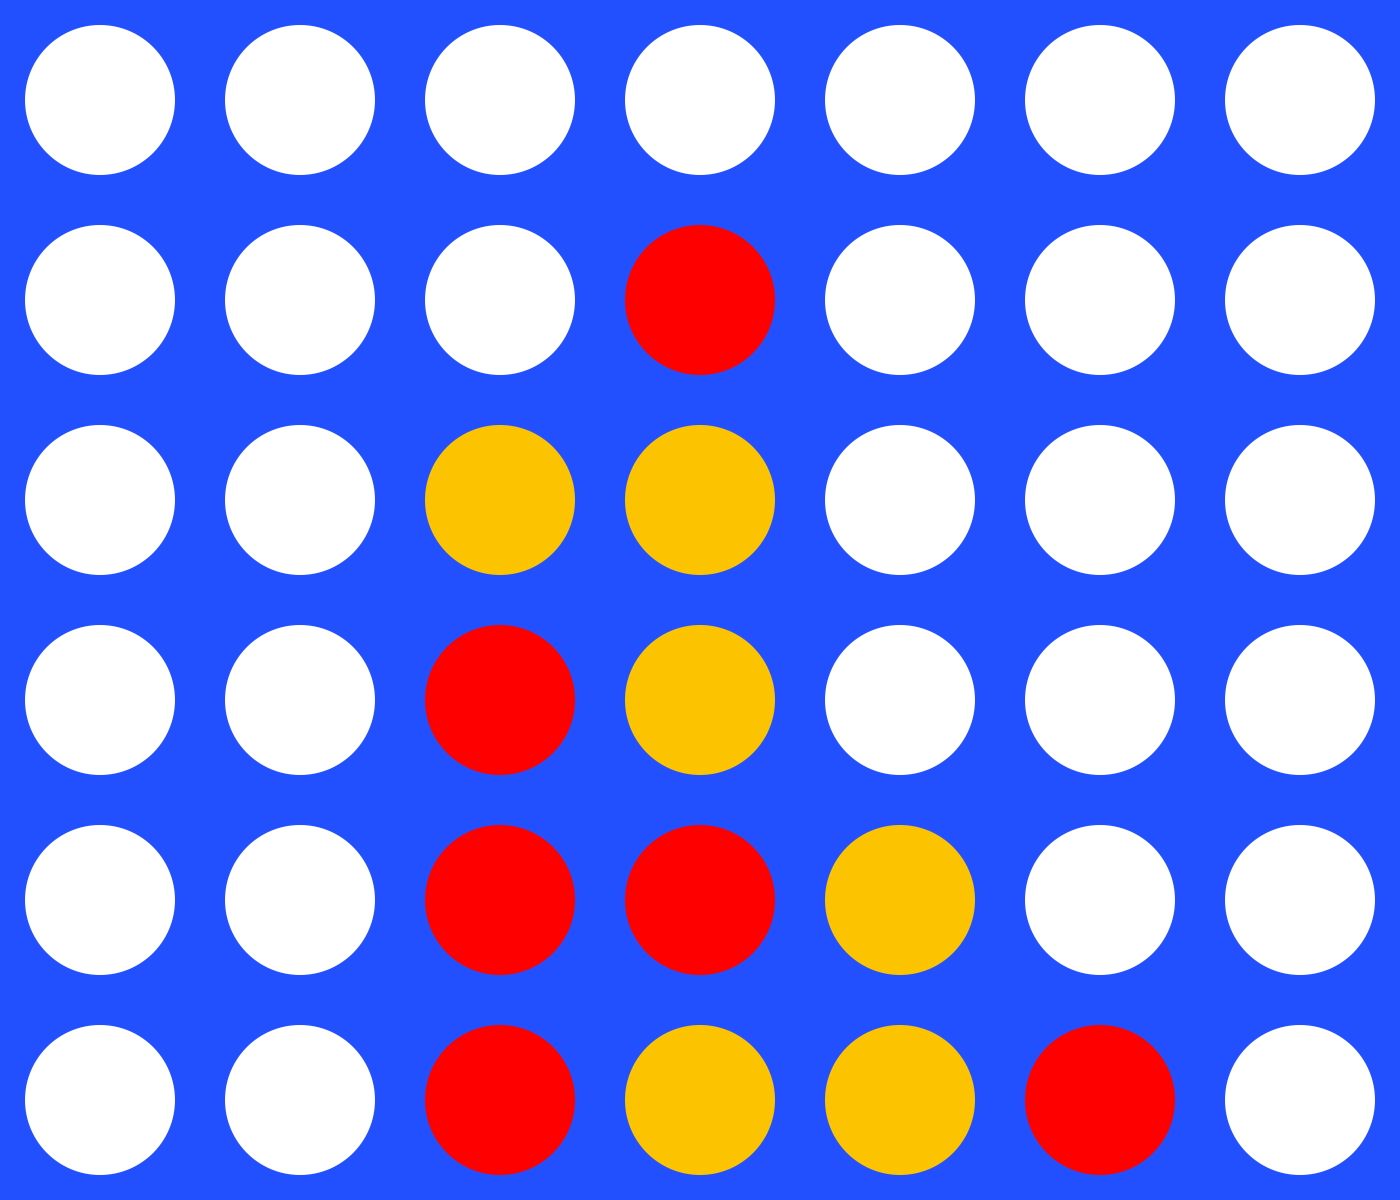
\includegraphics[width=0.5\textwidth]{connectFourExample}
\captionof{figure}{}
\label{fig:connect4ImageOne}
\end{center}

If red is the current player then:
\[
X = \left[
\begin{matrix}
\mathColor{black}{0} & \mathColor{black}{0} & \mathColor{black}{0} & \mathColor{black}{0} & \mathColor{black}{0} & \mathColor{black}{0} & \mathColor{black}{0}\\
\mathColor{black}{0} & \mathColor{black}{0} & \mathColor{black}{0} & \mathColor{red}{1}     & \mathColor{black}{0} & \mathColor{black}{0} & \mathColor{black}{0}\\
\mathColor{black}{0} & \mathColor{black}{0} & \mathColor{\gold}{0} & \mathColor{\gold}{0} & \mathColor{black}{0} & \mathColor{black}{0} & \mathColor{black}{0}\\
\mathColor{black}{0} & \mathColor{black}{0} & \mathColor{red}{1}     & \mathColor{\gold}{0} & \mathColor{black}{0} & \mathColor{black}{0} & \mathColor{black}{0}\\
\mathColor{black}{0} & \mathColor{black}{0} & \mathColor{red}{1}     & \mathColor{red}{1}     & \mathColor{\gold}{0} & \mathColor{black}{0} & \mathColor{black}{0}\\
\mathColor{black}{0} & \mathColor{black}{0} & \mathColor{red}{1}     & \mathColor{\gold}{0} & \mathColor{\gold}{0} & \mathColor{red}{1}     & \mathColor{black}{0}\\
\end{matrix}
\right]
\]\[
Y= \left[
\begin{matrix}
\mathColor{black}{0} & \mathColor{black}{0} & \mathColor{black}{0} & \mathColor{black}{0} & \mathColor{black}{0} & \mathColor{black}{0} & \mathColor{black}{0}\\
\mathColor{black}{0} & \mathColor{black}{0} & \mathColor{black}{0} & \mathColor{red}{0}     & \mathColor{black}{0} & \mathColor{black}{0} & \mathColor{black}{0}\\
\mathColor{black}{0} & \mathColor{black}{0} & \mathColor{\gold}{1} & \mathColor{\gold}{1} & \mathColor{black}{0} & \mathColor{black}{0} & \mathColor{black}{0}\\
\mathColor{black}{0} & \mathColor{black}{0} & \mathColor{red}{0}     & \mathColor{\gold}{1} & \mathColor{black}{0} & \mathColor{black}{0} & \mathColor{black}{0}\\
\mathColor{black}{0} & \mathColor{black}{0} & \mathColor{red}{0}     & \mathColor{red}{0}     & \mathColor{\gold}{1} & \mathColor{black}{0} & \mathColor{black}{0}\\
\mathColor{black}{0} & \mathColor{black}{0} & \mathColor{red}{0}     & \mathColor{\gold}{1} & \mathColor{\gold}{1} & \mathColor{red}{0}     & \mathColor{black}{0}\\
\end{matrix}
\right]
\] For clarification, the numbers are coloured in the same colour as the stones at that position. After stacking \(X\) and \(Y\), \(i_n\) is:
\[
i_n = \left[
\begin{matrix}
\mathColor{black}{[0,0]} & \mathColor{black}{[0,0]} & \mathColor{black}{[0,0]} & \mathColor{black}{[0,0]} & \mathColor{black}{[0,0]} & \mathColor{black}{[0,0]} & \mathColor{black}{[0,0]}\\
\mathColor{black}{[0,0]} & \mathColor{black}{[0,0]} & \mathColor{black}{[0,0]} & \mathColor{red}{[1,0]}     & \mathColor{black}{[0,0]} & \mathColor{black}{[0,0]} & \mathColor{black}{[0,0]}\\
\mathColor{black}{[0,0]} & \mathColor{black}{[0,0]} & \mathColor{\gold}{[0,1]} & \mathColor{\gold}{[0,1]} & \mathColor{black}{[0,0]} & \mathColor{black}{[0,0]} & \mathColor{black}{[0,0]}\\
\mathColor{black}{[0,0]} & \mathColor{black}{[0,0]} & \mathColor{red}{[1,0]}     & \mathColor{\gold}{[0,1]} & \mathColor{black}{[0,0]} & \mathColor{black}{[0,0]} & \mathColor{black}{[0,0]}\\
\mathColor{black}{[0,0]} & \mathColor{black}{[0,0]} & \mathColor{red}{[1,0]}     & \mathColor{red}{[1,0]}     & \mathColor{\gold}{[0,1]} & \mathColor{black}{[0,0]} & \mathColor{black}{[0,0]}\\
\mathColor{black}{[0,0]} & \mathColor{black}{[0,0]} & \mathColor{red}{[1,0]}     & \mathColor{\gold}{[0,1]} & \mathColor{\gold}{[0,1]} & \mathColor{red}{[1,0]}     & \mathColor{black}{[0,0]}\\
\end{matrix}
\right]
\]
\paragraph{Neural Network Architecture} 
\label{sec:NeruralNetworkArchitecture}
The neural network used by Alpha Zero consists of three main sub-modules, namely the residual tower, the value head and the policy head. The residual tower's purpose is to preprocess the data for the two heads. The value head determines the value \(v\) from the output of the residual tower. While the policy head computes the policy \(p\). The residual tower consists of a convolutional block followed by six residual blocks.\\
In my code, the convolutional block consists of the following: 
\begin{enumerate}
\item A convolutional layer consisting of 75 filters with a kernel size of 3 x 3
\item Batch normalization \cite{ioffe2015batch}
\item A non-linear rectifier (LeakyReLU).
\end{enumerate}
Every residual block consists of the following modules:
\begin{enumerate}
\item A convolutional layer consisting of 75 filters with a kernel size of 3 x 3
\item Batch normalization
\item A non-linear rectifier (LeakyReLU)
\item A convolutional layer consisting of 75 filters with a kernel size of 3 x 3
\item Batch normalization
\item Batch normalization outputs are added to the block's input.
\item A non-linear rectifier (LeakyReLU)
\end{enumerate}
Outputs are then passed to the value and policy head of the network for further evaluation.
I used a value head consisting of the following modules:
\begin{enumerate}
\item A convolutional layer consisting of 10 filters with a kernel size of 1 x 1
\item A fully connected layer of size 210
\item A non-linear rectifier (LeakyReLU)
\item A fully connected layer of size 1
\item \(tanh\) activation function
\end{enumerate}
My policy head consists of the following modules:
\begin{enumerate}
\item A convolutional layer consisting of 2 filters with a kernel size of 1 x 1
\item A fully connected layer of size 42
\item A LeakyReLU activation function
\end{enumerate}
The output of the policy head \(p_{pre}\) is then masked with the allowed actions to form \(p_{masked}\) in such a way that \(p_{masked}\) is \(-1000\) for all non-allowed actions. Finally, \(p_{masked}\) is passed throught the softmax function to form \(\pi\):
\begin{equation}\label{eq:nn:policyDefinition}
\pi = \text{softmax}(p_{masked})
\end{equation}

\paragraph{Model Training}\label{sec:Methods:NN:A0:Training}
Training is performed in batches of \(\batchSize\) states. Both heads are updated using \(mse\) (Mean-squared-error). In the policy network, all non-legal actions are ignored. This avoids unnecessary updating of the neural network. The value of the value head, the neural network is trained to predict for a certain MCTS node \(n\), is equivalent to 1 if the player who took an action at node \(n\) did win, \(-1\) if that player did lose and \(0\) if the game ended in a tie. The policy \(p_{a}\) to train for, for a given legal action \(a\in \mathbb A(n)\) is:
\begin{equation} \label{eq:NN:policy_computation}
p_{a} = \frac{N(n, a)}{\sum_{b\in \mathbb A(n)} N(n, b)}
\end{equation}
For non legal actions \(a \in (\mathbb A_{possible} - \mathbb A(n))\), \(p_{a}\) is defined as:
\begin{equation} \label{eq:NN:policy_computation_nonlegal}
p_{a} = p_{pre_{a}}
\end{equation}ˇ

\subsection{Training loop}
The Alpha zero training loop consists of data generation, training and testing. During data generation, data is generated, that is then used to train the neural network. After every training session, the new model is evaluated against the old one, to determine if it is better. If this is the case, the new model is used to generate data, if not, the old one generates data again and may be replaced after the next round.
\subsubsection{Data generation}
The data used to train the neural network is generated by letting the best agent play several games against itself, until enough data has been generated to allow for training. In every game, at every game state, the MCTS performs 50 simulations. Once the simulations are done the action is chosen.
\paragraph{Action selection}\label{sec:training:actionSelection}
There are two methods for action selection for a given node \(n_t\): deterministic and probabilistic. The first will always return the action \(a = argmax(N(a)), a\in\mathbb A(n_t)\) of the most traversed edge, while the second will return a random action where the probability of selecting an action \(a_i \in \mathbb A(n_t)\) is:
\begin{equation} \label{eq:ActionSelection:Probabilistic}
\mathcal P(X=a_i, n_t) = \frac{N(a_i)}{\sum_{j \in \mathbb A(n_t)} N(j)}
\end{equation}
(\(\mathbb A(n_t)\) are the allowed actions for state \(n_t\).) Action selection during the training phase shall initially be probabilistic, and deterministic later on. The handover point shall be defined as the configurational constant 'probabilistic\_moves' \(\in \mathbb N^+\). During games outside the training loop's data generation phase, actions are always selected deterministically.
 \paragraph{Memory}
\label{sec:memory}
The memory is used to store game states, after they where generated, but before they are used to train the neural network.
It stores a certain amount of memory elements. A memory element consists of a gamestate \(g \in \mathbb G\), its action values \(v \in \mathbb R^{|\mathbb A|}\) and the true reward \(r \in \mathbb \{\pm1, 0\}\) = \(R(g, a)\) where \(a\) is the action taken during play at that game state. The memory stores memory elements in a long list. After an action has been selected, but before any updates to the game simulation are made, the current game state is passed to temporary memory along with its action values \(v\). Together they create a new memory element. This element's \(r\) is currently undefined. \(v\) is defined as: 
\begin{equation} \label{eq:Memory:ActionValuesDefinition}
v_a = 
\begin{cases}
\mathcal P(X=a, \mathcal N(g)) & a \in \mathbb A(g)\\
p_{pre_a} &
\end{cases}
\end{equation}
\(\mathbb A(g)\) is the set of all legal actions. \(p_{pre}\) is defined in \sectionref{sec:NeruralNetworkArchitecture}, and is used for all non legal actions. \(P\) is defined in \equationref{eq:ActionSelection:Probabilistic}.

\paragraph{Memory update}\label{sec:memoryUpdate}
Once the game is over, the winning player is determined and the value \(r\) of every memory element in the temporary memory is updated. \(r\) is 1 if the player taking an action at that state won, -1 if he lost and 0 if the game ended in a draw. The updated states are then passed to memory.

\subsubsection{Model Training}
Once the memory size exceeds 30'000 states, the self-playing stops. Batches of \(\batchSize\) states are then randomly taken from all the states in the memory and used to train the neural network as described in \sectionref{sec:Methods:NN:A0:Training}.

\subsubsection{Model evaluation}\label{sec:modelEvaluation}
In order to train the neural network, the "best player" generates data used to train the current network.
After every time the current neural network has been updated, it plays \(20\) games against the best player. If it wins more than \(1.3\) times as often as the current best player, it is considered better. If this is the case, the neural network of the "current player" is saved to file and the old "best player" is replaced with the "current player" to become the new "best player". It is advantageous to force the network to win \(1.3\) times as often as that reduces the chance of the network just getting lucky. 
\section{Evaluation}\label{sec:evaluation}
To give us an idea of how good a player is, it would be useful to express performance using a single number. This number should not only give us a ranking but also allow for predictions of the winner of a game between two players and thus give us a measure of the relative strength of the players. One such rating method is the so called elo-rating method. \cite{elo1978rating}
\subsection{Elo-rating} \label{sec:Evaluation:elo-rating}
The elo-rating system assigns every player \(p\) a number \(r_p \in \mathbb{R}\). In general, the larger \(r_p\) the better the player. More specifically, given two players \(a\) and \(b\) with elo-ratings \(r_a\) and \(r_b\), the expected chance \(E\) of \(a\) winning against \(b\) is \cite{silver2018general}:
\begin{equation} \label{eq:elo_pred}
E = \frac{1}{1 + e^{(r_b-r_a)/400}}
\end{equation}
\begin{center}
\includesvg[width=0.8\columnwidth]{images/elo}
\captionof{figure}{elo-rating win probability for \(r_b = 0\)}
\end{center}
This function describes a sigmoid curve. This makes sense, because if the players have major strength discrepancies \(E\) converges to \(1\) or \(0\). When \(a\) and \(b\) play a game against each other, \(a\)'s elo rating is updated as follows\cite{elo1978rating}:

\begin{equation} \label{eq:elo_update}
r_{a_{n+1}} = r_{a_n} + K(W - E)
\end{equation}
with:
\begin{description}
\item \(r_{a_{n+1}}\) the new rating for the player.
\item \(r_{a_n}\) the current rating of the player.
\item \(W = s_a\) which is defined by equation \ref{eq:elo_score} where \(a\) is the player to be updated.
\item \(E\) the expected chance of winning, see equation \ref{eq:elo_pred}.
\item \(K\) is a constant controlling the sensitivity of the update function.
\end{description}
However, to avoid slow convergence of elo-ratings, a more direct formula is used to approximate the rating of an agent \(a\). This is done by playing a predetermined amount of games against player \(b\) whose elo-rating \(r_b\) is known and unchanged throughout this process. First, \(a\) and \(b\) play a predetermined amount of games \(m\) and the score \(s_a\) of \(a\) is computed as \cite{elo1978rating}:
\begin{equation} \label{eq:elo_score}
s_a = \frac{1}{m}\sum\left\{
\begin{array}{ll}
1 &              a\textrm{ wins} \\
\frac{1}{2} & \textrm{tie}\\
0 &              a\textrm{ looses}\\
\end{array}
\right.
\end{equation}
Assuming that this is the probability of \(a\) winning against \(b\), \(a\)'s elo-rating can be computed by solving equation \ref{eq:elo_pred} to \(r_a\) \imgRef{fig:eloInv}:
\begin{equation} \label{eq:elo_back}
r_a = r_b - ln\left(\frac{1-s_a}{s_a}\right) \cdot 400
\end{equation}
\begin{figure}
\center
\includesvg[width=0.8\columnwidth]{images/elo_back}
\captionof{figure}{elo inverse function for \(r_b = 0\)}
\label{fig:eloInv}
\end{figure}
Since a ranking of all the agents already exists (see \sectionref{sec:modelEvaluation}), an agent's elo-rating can be computed by playing against an older version and then using equation \ref{eq:elo_back} to determine its elo-rating. 
\subsubsection{Relativity of the Elo-rating}
The only problem is that elo is a relative rating. The rating of any other agent depends on its performance against other agents and their elo-ratings. Therefore, one must give the system a base rating for at least one predefined agent. In this case, there are no previously known elo-rated agents I could find, so I defined the untrained agent's elo-rating as 100. All other elo-ratings are relative to that.

\subsection{Elo results}
The rating \(r_i\) of any agent version \(i\) must in general be greater than the rating of the last version \(r_i > r_{i-1}\). Furthermore, the expected minimal increase in rating \(\Delta r_{min} = r_i - r_{i-1}\) is:
\begin{equation}\label{eq:deltaRCalculation}
\Delta r_{min} = -ln\left(\frac{1- \Delta s_i}{\Delta s_i}\right)\cdot 400
\end{equation}
Where \(\Delta s_i\) is the minimal expected chance of agent \(i\) beating agent \(i-1\).
As a certain scoring threshold \(\theta = 1.3\) was used during training to minimize the effect of noise in the evaluation, a prediction of \(s_i\) can be made. Given that \(s_i\) and \(s_{i-1}\) are the scores of agents \(i\) and \(i-1\), that play aginst each other, then by definition:
\begin{equation}\label{eq:scoreSumm}
s_i + s_{i-1} = 1
\end{equation}
Let \(w_i\) be the win count of agent \(i\) over game count.\\
Let \(d_i\) be the draw count over game count.\\
Let \(l_i\) be the loose count of agent \(i\) over game count.\\
Then:
\begin{align}
s_i &= w_i + \frac{d_i}{2}\\
s_{i-1} &= l_i + \frac{d_i}{2}
\end{align}
Then due to \(\theta\):
\begin{equation}
w_i \geqslant l_i \theta
\end{equation}
And by extension:
\begin{equation}
s_i \geqslant s_{i-1}
\end{equation}
Under the assumption, that there are no ties:
\begin{equation}\label{eq:scoregeq}
s_i \geqslant s_{i-1} \cdot \theta
\end{equation}
Let \(s_{min_i}\) be the minimal possible \(s_i\) (assuming no ties). Using \quickeq{eq:scoregeq} and \quickeq{eq:scoreSumm}:
\begin{align}
\left|\begin{aligned}
s_i + s_{i-1} &= 1\\
s_i                 &= s_{i-1}\theta
\end{aligned}\right|\\
\implies s_i = \frac{\theta}{1+\theta}\label{eq:siByTheta}
\end{align}
For \(\theta = 1.3\) this means that the expected average change in rating \(\Delta r\) using \quickeq{eq:siByTheta} and \quickeq{eq:deltaRCalculation}:
\begin{equation}
\Delta r \geqslant -ln\left(\frac{1}{\theta}\right)\cdot 400 = \Delta r_{min} \cong 105
\end{equation}
Collected data shows this to be true \imgRef{img:eloByVersion}. The same data shows that the average \(\Delta r \) is in fact roughly \(\FittedEloRaiting\), which would equate to a \(\theta\) of

\begin{equation}
\theta = \frac{1}{e^{\frac{-\Delta r}{400}}} \cong \FittedScoringThreshold
\end{equation}
\begin{center}
	\includesvg[width=0.9\textwidth]{eloRaitingByVersion}
	\captionsetup{width=.8\linewidth}
	\captionof{figure}{Elo-rating of agents based on their version along with the expected minimal rating \(\Delta r_{min}\) and the best fitted rating \(\Delta r\).}
	\label{img:eloByVersion}
\end{center}

\section{Implementation}
I began by implementing the MCTS and neural network seperately. First, I tried using Tensorflow for the neural network evaluation, but its C++ API is nearly undocumented and very complicated to use. So I setteled for Pytorch. With that solved, I implemented the basic training loop and ran the algorithm. This is when the problem of insufficent computational resources occurred. In an attempt to solve this, I ran the program over google cloud platform and moved model evaluation to the GPU. Furthermore, I made game simulation and data generation asynchronous to avoid CPU/GPU downtime while the other is computing. Additionally, I created two python GUI's and one C++ UI that comunicate with a C++ AI server to allow humans to play against the AI. Because the AI server was turned off most of the time but I still wanted to access the elo data and game logs, I created a dedicated data server to store this information. Then, because the AI server running on google cloud platform changes IP a lot, I created a webpage on a webserver, to redirect the clients to the right server. When I aquired a computer capable of handling the AI, a lot of this work became redundant. I also implemented a neural network in numpy and created supervised and unsupervised learning examples.
\section{Conclusion}
%In conclusion the algorythem works, and is able to learn to play connect4 at a level better than any human I could find. Some improvements can still be made, but in generall, Im rather happy with the results. If I were to ever do this again, I would stick with python.
I very much enjoyed the development of the AI as well as deriving the mathematics behind neural networks. Coding was a lot of fun though the endless debugging was painful. Performance issues were a major part of my concern. Solving these was an interesting experience. Working on asynchronous programs of this scale was a new experience for me, and it worked quite well.
As a result, I successfully developed an AI-based computer program that plays connect4, and has beaten every human so far that it played against.
I am very happy with the results. However, if I were ever to do this again, I would stick to python.
\\
Some improvements could be made - like the following
\subsection{Improvements}
\begin{itemize}
\item The algorithm could be completely rewritten to allow for training on TPU's (tensor processing units).
\item Process distribution could be improved to allow for training of the AI on multiple GPU's.
\item The algorithm could be tested for different games and other configurations.
\item Since most of the time is spent on running neural network simulations, process efficiency could be improved by not only updating MCTS graphs to the current node, but all the way back to the root. Furthermore, not only updating the path but every possible path back would increase efficency even further - at least in theory. 
\end{itemize}

\newpage
\bibliographystyle{plain}
\bibliography{bibliography}

\newpage
\section*{Acknowledgements}
\begin{itemize}
\item Leonie Scheck, Frederik Ott, Nico Steiner, Wolfgang Wandhoven for assisting in evaluating the AI against human players and providing feedback.
\end{itemize}

\newpage
\section{Appendix: Further definitions}
\subsection{Hadamard product}\label{sec:hadamerd_product}
Let \(A\) and \(B\) be 2 \(m \times n\) matrices. For all \(i \in [1, m]\cap\mathbb N\) and \(j \in [1, n]\cap\mathbb N\)
the hadamard product \(A \circ B\) is defined as:
\begin{equation} \label{eq:defs:Hadamard product}
\left(A \circ B\right)_{ij} = A_{ij} \cdot B_{ij}
\end{equation}
For example consider the following \(2 \times 3\) matrices:
\[
\left[
\begin{array}{ll}
a_{11} & a_{12} \\
a_{21} & a_{22} \\
a_{31} & b_{32} \\
\end{array}
\right] \circ 
\left[
\begin{array}{ll}
b_{11} & b_{12} \\
b_{21} & b_{22} \\
b_{31} & b_{32} \\
\end{array}
\right] = 
\left[
\begin{array}{ll}
a_{11}b_{11} & a_{12}b_{12} \\
a_{21}b_{21} & a_{22}b_{22} \\
a_{31}b_{31} & a_{32}b_{32} \\
\end{array}
\right]
\]\\

\subsection{Inner Product}
\subsubsection{Matrices}
Let \(A\in \mathbb{R}^{m \times n}\) and \(B\in \mathbb{R}^{m \times n}\) be two \(n \times m\) matrices. \\Let their Inner Product \(A\diamond B\;:\; \mathbb{R}^{m \times n},~\mathbb{R}^{m \times n} \to \mathbb{R}\) be defined as:
\begin{equation} \label{eq:defs:Inner_product}
A \diamond B = \sum_{i=1}^{m}\sum_{j=1}^{n} A_{ij}B_{ij} = \sum_{i=1}^{m}\sum_{j=1}^{n} (A \circ B)_{ij}
\end{equation}
For example consider the following \(2 \times 3\) matrices:
\[
\begin{bmatrix}
a_{11} & a_{12} \\
a_{21} & a_{22} \\
a_{31} & b_{32} \\
\end{bmatrix}
\diamond
\begin{bmatrix}
b_{11} & b_{12} \\
b_{21} & b_{22} \\
b_{31} & b_{32} \\
\end{bmatrix}
= \;
\begin{array}{ll}
     a_{11}b_{11} + a_{12}b_{12} + a_{21}b_{21}\\
+~a_{22}b_{22} + a_{31}b_{31} + a_{32}b_{32} 
\end{array}
\]

\subsubsection{\(n\)-dimensional Tensors}
Let \(A \in \mathbb{R}^{m \times \dots}\) and \(B \in \mathbb{R}^{m \times \dots}\) be two \(n\) dimensional \(m \times \dots\) tensors with \(n > 2\)\\
Let the Inner product \(A \diamond B : \mathbb{R}^{m \times \dots}, \mathbb{R}^{m \times \dots} \to \mathbb{R}\) be defined as:
\begin{equation}\label{eq:defs:Inner_product_3d}
A \diamond B = \sum_{i=0}^{m} A_{i} \diamond B_{i}
\end{equation}
%
%%sidewaysfigure
%\begin{sidewaysfigure}[ht]
%    \centering
%	\captionsetup{width=.9\linewidth}
%    \includesvg[width=\columnwidth]{images/MCTS-steps.svg}
%		\caption[width=0.7\columnwidth]{MCTS simulation steps. In this diagram, the numbers in the node represent \(Q\) and the number on the arrow is \(P\). The red nodes are leaf nodes and the green one is the leaf node \(n_L\). During the \textbf{selection} phase, \(\sigma\) is used to find successive nodes until the node \(n_L\) is reached. This is shown with the arrows. During the \textbf{expansion} phase, new nodes and edges are added for all possible legal actions at the node \(n_L\). The \textbf{evaluation} phase gives the new nodes the following values \(Q = 0\) and \(P = \pi_a\). The value of the leaf \(v\) is then used during the \textbf{backfill} phase to update the \(Q\)'s of all nodes traversed during selection.}
%		\source{modified from \url{https://en.wikipedia.org/wiki/File:MCTS-steps.svg}\\File available under \href{https://creativecommons.org/licenses/by-sa/4.0/deed.en}{Creative Commons Attribution-Share Alike 4.0 International} at %\url{https://wandhoven.ddns.net/edu/AlphaZeroTheory/images/MCTS-steps.svg}}
%	\label{MCTS-simulation}
%\end{sidewaysfigure}

\subsection{Submatrix}
\label{sec:Ref:submatrix}
Let \(M \in\mathbb R^{m\times n\times o}\) be a tensor of size  \(m\times n\times o\).\\
Let \(\left<\right>_{x\times y,\,ab}\) be the matrix slicing operator. \(x\times y\) is the size of the submatrix the operation should output. \(ab\) is the top left position of the submatrix within the outer matrix.  For the operation to be defined, the following must be true: \(x \in [1, m[\cap\mathbb N\), \(y \in [1, n[ \cap\mathbb N\), \(a  \in [1, m-x+1]\cap\mathbb N\) and \(b \in [1, n-y+1]\cap\mathbb N\). The submatrix \(\left<M\right>_{x\times y,\,ab}\) is defined as:
\begin{equation}
\left<M\right>_{x\times y,\,ab} = 
\left[
\begin{matrix}
[M_{ab1},\dots,M_{abo}] & \dots & [M_{(a+x-1)b1},\dots,M_{(a+x-1)bo}]\\
\vdots &  \ddots & \vdots\\
[M_{a(b+y-1)1},\dots,M_{a(b+y-1)o}] & \dots & [M_{(a+x-1)(b+y-1)1},\dots, M_{(a+x-1)(b+y-1)o}]\\
\end{matrix}\right]
\end{equation}

\subsection{Vectorization}  \label{sec:ref:vectorization}
``[\dots] the vectorization of an \(m \times n\) matrix \(A\), denoted \(\text{vec}(A)\), is the \(mn \times 1\) column vector obtained by stacking the columns of the matrix A on top of one another''\cite{vectorization_2021}: 
\begin{equation}\label{eq:ref:vectorization}
\text{vec}(A) = \left[
A_{11}\,\dots\,A_{1m}\,A_{21}\,\dots \,A{2m}\,\dots\,A_{n1}\,\dots\,A{nm}
\right]^T
\end{equation}
For example, the \(3\times 2\) matrix \(A=\left[
\begin{matrix}
a & b & c\\
d & e & f\\
\end{matrix}
\right]\) vectorizes to
\[
\text{vec}(A) = \left(
\begin{matrix}
a\\
b\\
c\\
d\\
e\\
f\\
\end{matrix}
\right)
\]
\subsubsection{Tensor Vectorization}\label{sec:ref:vectorization:tensor}
Let \(T \in \mathbb R^{n \times\dots}\) be a m-dimensional Tensor.
Let \(vec(T)\) be defined as:
\begin{equation}
vec(T) = vec(T_0) \frown vec(T_1) \frown \dots \frown vec(T_n)
\end{equation}
Where \(\frown\) is defined defined in \sectionref{sec:ref:vectorConcatination}. For those familiar with python's numpy library, \(vec\) is equivalent to numpy.flatten.

\subsection{Vector Concatination}\label{sec:ref:vectorConcatination}
Vector Concatination of two vectors \(v\) and \(u\) of dimensions \(n_v\) and  \(n_u\), denoted \(v\frown u\), is the \(n_v + n_u\) dimensional vector obtained by placing both vectors one on top of the other.
\begin{equation} \label{eq:ref:vecConcatination}
v\frown u = \left(
\begin{matrix}
v_1\\
\vdots\\
v_{n_v}\\
u_1\\
\vdots\\
u_{n_u}\\
\end{matrix}
\right)
\end{equation}\\

\subsection{Source Code Locations}
The source code can be found in the following github repositories:
\begin{itemize}
\item AI, AI-Server, data server and UI's: \url{https://github.com/JulianWww/AlphaZero} 
\item Supervised and unsupervised learning demos: \url{https://github.com/JulianWww/Matura-AlphaZero-demos}
\item Neural network in python: \url{https://github.com/JulianWww/NeuralNetwork}
\item This Document: \url{https://github.com/JulianWww/MaturArbeitAlphaZero}
\end{itemize}
\end{document}
